\documentclass[18pt]{article}
\usepackage{geometry}
\usepackage{mathexam}
\usepackage{amsmath}
\usepackage{graphicx}
\begin{document}
\begin{titlepage}
   \vspace*{\stretch{1.0}}
   \begin{center}
      \Large\textbf{Mathematical model for CAD Software}\\
      \large\textit{Rahul Bansal and GSM Rishikesh Reddy}
   \end{center}
   \vspace*{\stretch{2.0}}
\end{titlepage}
\title{3D Model to 2D projections on any Plane}
\maketitle
\section{Brief Introduction}
\large{In this model we have two major tasks first being that we are a given 3 Dimensional figure and an arbitrary plane in 3D space and we are required to obtain the projection of the 3D figure on that plane as shown in the figure bellow.}\\{}\\{}\\{}\\{}\\
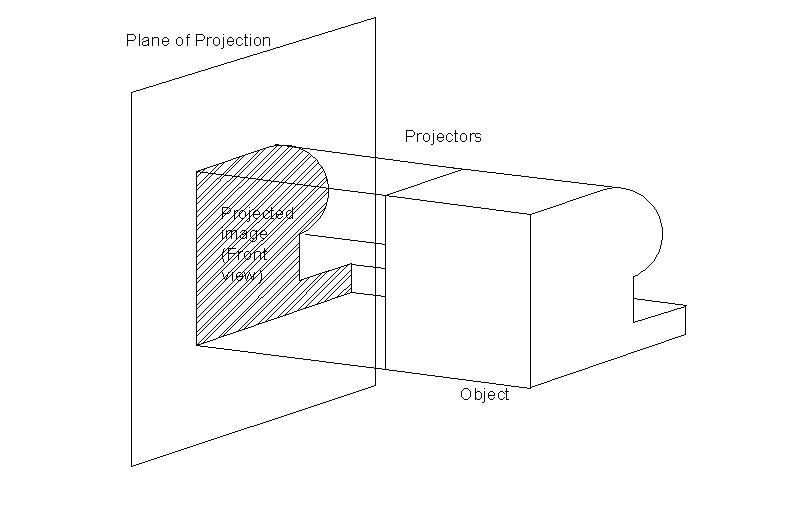
\includegraphics[scale=0.75]{3d_to_2d.png}
\large{The second task of this model is that we will be given orthographic views of a 3D object and we will have to construct the 3D object using the given orthographic views as shown in the image bellow. }\\{}\\{}\\{}\\{}\\
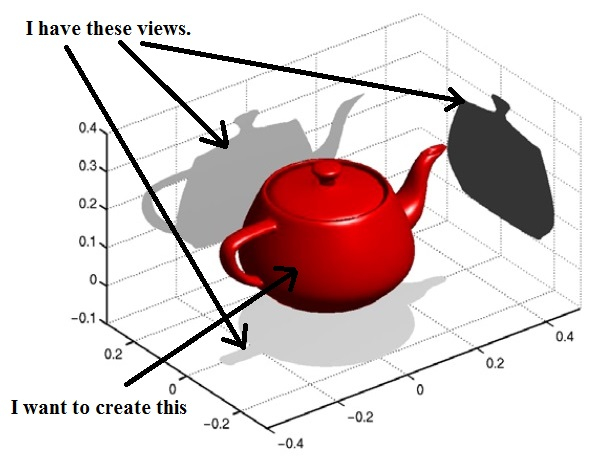
\includegraphics[scale=0.75]{2d.png}\\{}\\
\section{Assumptions of our 3D model}
\large{We define a minimum unit of length for all the figures which can be drawn using this software, as say k. So in this model the user cannot input two points that have their distance less than order of k.\\
When any user inputs some 3D figure into our model we can convert that figure into set of 3D coordinates or 3D vectors,
$\Vec{v}=\begin{bmatrix} 
x\\
y\\
z
\end{bmatrix}$ as follows-\\{}\\
We take a number k' which is a fraction of k. Assume that the 3D figure is between the dimensions $X*Y*Z$. So we have to label  $\dfrac{X*Y*Z}{(k')^3}$  number of points in the 3D space. \\All the points that are inside in the figure input by the user are labelled as 1 and others as 0. So now we will have a set of points that have the label 1. \\
Now our goal is to convert this set of 3D vectors to a set of 3D vectors that lie on the plane on which the projection has to be taken which satisfy a particular equation of that plane.\\$$ ax + by + cz = d$$ }\\
\section{Projection of a point on a Plane}
\large{In this section we see how to take projection of any point in 3D space on a given 2D plane.\\
A point $(x_{o},y_{o},z_{o})$ can be represented as a vector, $\Vec{v_{o}}=\begin{bmatrix} 
x_{o}\\
y_{o}\\
z_{o}
\end{bmatrix}$\\{}\\{}\\
General equation of a plane -      $ax + by + cz = d  $ where a,b,c,d $\in $ R\\{}\\
The normal vector of this plane is , $\Vec{N}=\begin{bmatrix} 
a\\
b\\
c
\end{bmatrix}$\\{}\\
The general equation of plane can be represented as  \Large{$\Vec{v^t}*\Vec{N} = d $}\\}{}\\
{For finding the projection of the vector $\Vec{v_{o}}$  we define a vector $\Vec{v}= t*\Vec{N} +  \Vec{v_{o}}$\\ , where l $\in $ R.
As projection of the point should satisfy the equation of Plane so substituting the $\Vec{v}$ in $\Vec{v^t}*\Vec{N} = d $ we will get a solution for t which will give the point of projection on the plane.
Solving this we get - $$ t = \dfrac{d - \Vec{{v_{o}}^t} * \Vec{N}}{\Vec{N^t} * \Vec{N}}$$\\
Substituting this value in $\Vec{v}= t*\Vec{N} +  \Vec{v_{o}}$ we get the required projection of the point $\Vec{v_{o}}$ on the plane $ax + by + cz = d  $ .
}

\section{Rotation of a 3D figure}
\large{Assume we have a 3D image in some specific orientation in 3D space. Now the user wants to rotate the given figure to some new orientation. By rotating the figure to a new orientation the coordinates of each of the point on the object will change and thus will the projection of the figure on the plane. So for obtaining the new projection, we the set of the new coordinates of the object after the rotation. For finding the new set of coordinates we make us of \textbf{Rotation Matrix.}\\
\textbf{Rotation Matrix} is a matrix that is used to perform a rotation in Euclidean space.\\
Rotation matrix in 2D can be written as -{}\\
$$ R(\theta) = \begin{bmatrix} 
\cos{\theta} & -\sin{\theta} \\
\sin{\theta} & \cos{\theta}
\end{bmatrix}$$\\
This matrix rotates points in the XY-plane counterclockwise through an angle $\theta$ about the origin of the Cartesian coordinate system. To perform the rotation using a rotation matrix R, the position of each point must be represented by a column vector $\Vec{v}$, containing the coordinates of the point. A rotated vector is obtained by using the matrix multiplication $R *\Vec{v} $. \\
$$\begin{bmatrix} 
x'\\
y'
\end{bmatrix} =\begin{bmatrix} 
\cos{\theta} & -\sin{\theta} \\
\sin{\theta} & \cos{\theta}
\end{bmatrix} \begin{bmatrix} 
x\\
y
\end{bmatrix}  $$\\
So the new coordinates (x',y') of the point (x,y) after rotation are,\\
$$x' = x \cos{\theta} - y \sin{\theta}$$
$$y' = x \sin{\theta} + y \cos{\theta}$$\\
The direction of vector rotation is counterclockwise if θ is positive (e.g. 90°), and clockwise if θ is negative (e.g. −90°). Thus the clockwise rotation matrix is found as
$$ R(-\theta) = \begin{bmatrix} 
\cos{\theta} & \sin{\theta} \\
-\sin{\theta} & \cos{\theta}
\end{bmatrix}$$\\
Now we have seen rotation in \textbf{2D} lets jump to the \textbf{3D} case.\\{}\\
\Large{\textbf{Basic Rotations}}{}\\{}\\
\large{A basic rotation (also called elemental rotation) is a rotation about one of the axes of a Coordinate system. The following three basic rotation matrices rotate vectors by an angle $\theta$ about the X, Y, or Z-axis, in three dimensions, using the right-hand rule—which codifies their alternating signs.The rotation matrices for rotation along an axis are -}\\
$$ R_{x}(\theta) = \begin{bmatrix} 
1 & 0 & 0 \\
0 & \cos{\theta} & -\sin{\theta}\\
0 & \sin{\theta} & \cos{\theta}
\end{bmatrix}$$\\
$$ R_{y}(\theta) = \begin{bmatrix} 
\cos{\theta} & 0 & \sin{\theta} \\
0 & 1 & 0\\
 -\sin{\theta} & 0 & \cos{\theta}
\end{bmatrix}$$\\
$$ R_{y}(\theta) = \begin{bmatrix} 
\cos{\theta} &- \sin{\theta} & 0 \\
\sin{\theta} & \cos{\theta} & 0 \\
0 & 0 & 1
\end{bmatrix}$$\\
For column vectors, each of these basic vector rotations appears counterclockwise when the axis about which they occur points toward the observer, the coordinate system is right-handed, and the angle θ is positive. $R_{z}$, for instance, would rotate toward the Y-axis a vector aligned with the X-axis.\\{}\\
\textbf{Generalized Rotation matrix} can be obtained from these three basic rotation matrices using matrix multiplication. For example,
$$R = R_{x}(\alpha)R_{y}(\beta)R_{x}(\gamma)$$\\
here R represents a rotation matrix for extrinsic rotation whose Euler angles are $\alpha,\beta,\gamma$ about axes X, Y, Z.\\
Hence if the user rotates the object by arbitrary angles $\alpha,\beta,\gamma$ we can always obtain a Rotation matrix corresponding to that rotation. So by matrix multiplication($R * \Vec{v}$) of set of coordinates with the Rotation matrix we will obtain a new set of coordinates which can then be projected on the required plane.
\section{Taking projection of the Object}
\large{Now we have all the mathematical tools required for the projection of the 3D object on any arbitrary plane. Let’s make a cube with dimensions in such a way that entire object lies in it. We divide the region of projection of the cuboid into points using the k’ parameter used earlier in obtaining the points. Let the projection of the cuboid have the area $X* Y $ . Then the total number of points to be labelled are $\dfrac{X∗ Y }{(k′)^2}.  $\\{}\\
Now we project each point of the object on the plane using the formula for the projection of a point on a plane. If we find the two points of the object  between which the point we are supposed to label lies, then we label the point as 1. Now we have a set of points labelled 1 on the plane which will together constitute the projection of the object on that plane.}
\section{Conversion of Orthographic views to 3D Object}
\large{In this case we will know which point corresponds to which other point in other orthogonal view. So if $(x_{1},y_{1})$ is a point labelled as 1 from a plane and $(y_{1},z_{1})$ be another which is labelled 1 from a different orthogonal plane. Now using this we label $(x_{1},y_{1},z_{1})$ as 1. For the other cases we label them as 0. Now we have a set of points $(x,y,z)$ which will together constitute the 3D object. }
}
\end{document}

\lar